%%%%%%%%%%%%%%%%%%%%%%%%%%%%%%%%%%%%%%%%%%%%%%%%%%%%%
%
%  Template
%  Beamer Presentation by Chris Bourke
%
%%%%%%%%%%%%%%%%%%%%%%%%%%%%%%%%%%%%%%%%%%%%%%%%%%%%%%%%%%%%%%%%%%%%%%%

\documentclass[]{beamer}
%\documentclass[handout]{beamer}

\geometry{papersize={16cm,9cm}}

% For handout version:
%\usetheme[hideothersubsections,slidenumbers]{UNLTheme}
\usetheme[hideothersubsections]{UNLTheme}
\usepackage{amssymb}
\input{StandardCommands}
\usepackage[linesnumbered,ruled,vlined]{algorithm2e}
\SetKwComment{Comment}{//}{}
\DontPrintSemicolon
\SetKwSty{textsc} %
%\SetAlFnt{\scriptsize} %
\SetKwInOut{Input}{Input} %
\SetKwInOut{Output}{Output} %
%\setalcapskip{1em} % changed to
\SetAlCapSkip{1em}
\setlength{\algomargin}{2em} %
%\Setvlineskip{0em} % changed to:
\SetVlineSkip{0em}

\usepackage{tikz}
\usetikzlibrary{fadings}
\usetikzlibrary{shapes.geometric,shapes.symbols}
\usetikzlibrary{calc,shapes.multipart,chains,arrows}
\usetikzlibrary{arrows.meta,calc,shapes.multipart,chains,arrows}
%\usetikzlibrary{calc,shapes.multipart,chains,arrows}
%%\usetikzlibrary{backgrounds}
\usetikzlibrary{backgrounds}
\usetikzlibrary{decorations.pathreplacing}
\usetikzlibrary{decorations.pathmorphing}
\tikzset{onslide/.code args={<#1>#2}{%
  \only<#1>{\pgfkeysalso{#2}} % \pgfkeysalso doesn't change the path
}}
\tikzset{temporal/.code args={<#1>#2#3#4}{%
  \temporal<#1>{\pgfkeysalso{#2}}{\pgfkeysalso{#3}}{\pgfkeysalso{#4}} % \pgfkeysalso doesn't change the path
}}

\tikzset{
    fading speed/.code={
        \pgfmathtruncatemacro\tikz@startshading{50-(100-#1)*0.25}
        \pgfmathtruncatemacro\tikz@endshading{50+(100-#1)*0.25}
        \pgfdeclareverticalshading[%
            tikz@axis@top,tikz@axis@middle,tikz@axis@bottom%
        ]{axis#1}{100bp}{%
            color(0bp)=(tikz@axis@bottom);
            color(\tikz@startshading)=(tikz@axis@bottom);
            color(50bp)=(tikz@axis@middle);
            color(\tikz@endshading)=(tikz@axis@top);
            color(100bp)=(tikz@axis@top)
        }
        \tikzset{shading=axis#1}
    }
}

\usepackage{multirow}
\usepackage{multicol}

\definecolor{steelblue}{rgb}{0.2745,0.5098,0.7059}
\hypersetup{
    colorlinks = true,
    urlcolor = {steelblue},
    linkbordercolor = {white}
}

\definecolor{mintedBackground}{rgb}{0.95,0.95,0.95}
\definecolor{mintedInlineBackground}{rgb}{.90,.90,1}

%\usepackage{newfloat}
\usepackage{minted}
\setminted{mathescape,
               linenos,
               autogobble,
               frame=none,
               fontsize=\small,
               framesep=2mm,
               framerule=0.4pt,
               %label=foo,
               xleftmargin=2em,
               xrightmargin=0em,
               startinline=true,  %PHP only, allow it to omit the PHP Tags *** with this option, variables using dollar sign in comments are treated as latex math
               numbersep=10pt, %gap between line numbers and start of line
               style=default, %syntax highlighting style, default is "default"
               			    %gallery: http://help.farbox.com/pygments.html
			    	    %list available: pygmentize -L styles
               bgcolor=mintedBackground} %prevents breaking across pages
               
\setmintedinline{bgcolor={mintedInlineBackground}}
\setminted[text]{bgcolor={},linenos=false,autogobble,xleftmargin=1em}

\tikzstyle{decision} = [diamond, draw, fill=yellow!20, 
    text width=6em, text badly centered, node distance=5cm, inner sep=0pt]
\tikzstyle{block} = [rectangle, draw, fill=blue!20, 
    text width=5em, text centered, node distance=5cm, minimum height=4em]
\tikzstyle{action} = [rectangle, draw, fill=green!20, 
    text width=5em, text centered, rounded corners, node distance=5cm, minimum height=4em]
\tikzstyle{line} = [draw, -latex']

\title[~]{Computer Science I}
\subtitle{Error Handling}
\author[~]{Dr.\ Chris Bourke\\ \email{cbourke@cse.unl.edu}} %
\date{~}

\begin{document}

\begin{frame}
  \titlepage
\end{frame}

\setbeamertemplate{section in toc}{\inserttocsectionnumber.~\inserttocsection}
\setbeamercolor{section in toc}{fg=black}
%\setbeamertemplate{subsection in toc}{~} %\inserttocsubsection\\}

\begin{frame}
  \frametitle{Outline}
%{\footnotesize
%\begin{NoHyper}
%  \tableofcontents[hideallsubsections]
%\end{NoHyper}
%}

\setbeamercolor{enumerate item}{bg=white,fg=black}
\setbeamercolor{item}{bg=white,fg=black}
\setbeamercolor{item projected}{bg=white,fg=black}
\setbeamercolor{enumerate subitem}{fg=red!80!black}
\setbeamertemplate{enumerate items}[default]
\begin{enumerate}
  \item Introduction
  \item Error Codes
  \item Defensive Programming
     %emphasize null pointer checks
     %demo with previous module's distance library
     %emphasize: in general, functions should NOT EXIT
     %emmphasize: in general, functions should not print error output
     %emphasize: look before you leap; error checking shoudl always be the first thing you do in a function
  \item Enumerated Types
  \item Unit Testing
\end{enumerate}

\end{frame}

\section{Introduction}

\begin{frame}
    \frametitle{}
    \framesubtitle{}
    
    \begin{center}
    {\Huge Part I: Introduction}\\
    {\Large ~}
    \end{center}

\end{frame}


\begin{frame}
    \frametitle{Error Handling}
    \framesubtitle{}

\begin{itemize}[<+->]
  \item Errors in computer systems are \emph{inevitable}
  \item Bugs vs.\ errors
  \item Bug: a flaw or defect in a computer program that causes it to produce an incorrect or unexpected result, or to behave in an unintended way
  \item Error: potential condition or state that can be reasonably anticipated by a programmer
  \item Bugs are flaws that should be resolved with rigorous \emph{testing}
\end{itemize}

\end{frame}


\begin{frame}[fragile]
    \frametitle{Errors}
    \framesubtitle{}


\begin{itemize}[<+->]
  \item Errors cannot be ``prevented'' only mitigated, anticipated, and \emph{handled}
  \item Common errors:
  \begin{itemize}
    \item Bad input leads to bad output (GIGO)
    \item Illegal operations: dividing by zero
    \item Dereferencing \mintinline{c}{NULL} pointers
    \item More general problems: missing file, limited resources (memory), bad password, no network connection, 
  \end{itemize}
  \item Some errors may be unexpected/catastrophic/fatal
  \item Others are \emph{recoverable}
\end{itemize}

\end{frame}


\begin{frame}[fragile]
    \frametitle{Error Handling}
    \framesubtitle{}


\begin{itemize}[<+->]
  \item Dealing with error conditions is called \emph{error handling}
  \item Two general approaches
  \item Defensive programming:
  \begin{itemize}
    \item Check for dangerous/illegal/invalid operations 
      before doing them; if an error would result, we ``choose'' not do to them
    \item We can then ``fail silently'' or communicate the type of error and
    let the calling function decide \emph{how to handle it}
    \item ``Look before you leap''
  \end{itemize}
  \item Exception handling
\end{itemize}

\end{frame}

\begin{frame}[fragile]
    \frametitle{Exception Handling}
    \framesubtitle{}  

\begin{itemize}[<+->]
  \item Modern programming support \emph{Exceptions}
  \item Exception: an \emph{event} during the execution of a program 
    that disrupts the normal control flow of the program
  \item Exceptions are \emph{thrown} and may be \emph{caught} (and handled)
  \item ``Go ahead and leap without looking, you'll be \emph{caught} if you fall''
  \item Many advantages to exception handling over defensive programming
  \item Not supported in C
\end{itemize}    

\end{frame}

\begin{frame}[fragile]
    \frametitle{Error Handling in C}
    \framesubtitle{}


\begin{itemize}[<+->]
  \item C generally uses defensive programming
  \item Error handling is generally on the function-level 
  \item Functions validate input, check for error conditions, etc.\ before proceeding
  \item If an error is detected, the function aborts and returns
  \item Error condition is communicated to the calling function via an \emph{error code}
  \item Error code: a number (integer) indicating the type of error (or none)
\end{itemize}

\end{frame}

\section{Error Codes}

\begin{frame}
    \frametitle{}
    \framesubtitle{}
    
    \begin{center}
    {\Huge Part II: Error Codes}\\
    {\Large ~}
    \end{center}

\end{frame}

\begin{frame}[fragile]
    \frametitle{Error Codes}
    \framesubtitle{}

\begin{itemize}[<+->]
  \item C provides a standard error library: \mintinline{c}{errno.h} (error number)
  \item Defines standard \emph{errors codes} and some (limited) utilities
  \item A global \mintinline{c}{int} variable named \mintinline{c}{errno} can be set by standard functions in the event of an error
  \item Value can be checked for an error ``state''
  \item Zero: no error
  \item Only three ``standard'' error codes:
  \begin{itemize}
    \item \mintinline{c}{EDOM} indicates an error in the domain of a function
    \item \mintinline{c}{ERANGE} indicates an error in the range of a function
    \item \mintinline{c}{EILSEQ} illegal byte sequence
  \end{itemize}
  \item Error codes defined via macros \mintinline{c}{#define}
\end{itemize}

\end{frame}

\begin{frame}
    \frametitle{EDOM}
    \framesubtitle{}

\mintinline{c}{EDOM}
\begin{itemize}[<+->]
  \item Error in the domain value of a function
  \item Functions map a \emph{domain} to a \emph{range}
  \item Domain is the set of all possible inputs
  \item In other words: illegal input
  \item Example: $\sqrt{x}$ is only defined for values $\geq 0$
  \item \mintinline{c}{sqrt(-1)} would result in an \mintinline{c}{EDOM} error
\end{itemize}
    
\end{frame}

\begin{frame}
    \frametitle{ERANGE}
    \framesubtitle{}

\mintinline{c}{ERANGE}
\begin{itemize}[<+->]
  \item Error in the range value of a function
  \item Range is the set of all possible outputs
  \item Illegal or aberrant output value from a function
  \item Example: $\log{(0)}$ is undefined (but converges to $-\infty$)
  \item \mintinline{c}{log(0)} would result in an \mintinline{c}{ERANGE} error
  \item Demonstration
\end{itemize}
    
\end{frame}


\begin{frame}
    \frametitle{POSIX Error Codes}
    \framesubtitle{}

\begin{itemize}[<+->]
  \item Portable Operating System Interface (POSIX) standard defines many more error codes
  \item Mostly for systems programming 
  \item Examples:
  \begin{itemize}
    \item No such file or directory
    \item Out of memory
    \item Network is down
  \end{itemize}
  \item Demonstration %\url{http://www.virtsync.com/c-error-codes-include-errno}
\end{itemize}

\end{frame}

\begin{frame}
    \frametitle{Exit Codes}
    \framesubtitle{}

\begin{itemize}[<+->]
  \item Similar: \emph{exit codes}
  \item When a program quits, it can ``return'' a value to the operating system
  \item Can be used externally to determine if a program was successful 
  \item Example: Segmentation Faults usually exit with an error code of 139
  \item Actual numbers are not standardized
  \item Two standard flags defined in \mintinline{c}{stdlib.h}
  \item \mintinline{c}{EXIT_FAILURE} (usually 1)
  \item \mintinline{c}{EXIT_SUCCESS} (usually 0, no error)
  \item Demonstration
\end{itemize}

\end{frame}


\section{Defensive Programming}

\begin{frame}
    \frametitle{}
    \framesubtitle{}
    
    \begin{center}
    {\Huge Part III: Defensive Programming}\\
    {\Large ~}
    \end{center}

\end{frame}

\begin{frame}
    \frametitle{Defensive Programming}
    \framesubtitle{}

\begin{itemize}[<+->]
  \item Don't generally use standard error codes for user-defined functions
  \item Can use the same approach: defensive error checking with error codes
  \begin{enumerate}
    \item Look before you leap: check for invalid state before a dangerous
    operation 
    \item If invalid, return an error code to communicate the \emph{type of error}
  \end{enumerate}
\end{itemize}
\end{frame}

\begin{frame}
    \frametitle{Defensive Programming}
    \framesubtitle{}

General design philosophy: 
\begin{itemize}[<+->]
  \item You \emph{communicate} the error to the calling function
  \item You \emph{don't} decide (dictate) what how to \emph{handle} the error
  \item The calling function is responsible for deciding what to do
\end{itemize}

\end{frame}

\begin{frame}
    \frametitle{Defensive Programming}
    \framesubtitle{}

Advantages:
\begin{itemize}[<+->]
  \item Makes your functions more flexible
  \item Leaves the decision making process to the user of the library
  \item Different error codes means the calling function can decide to apply different solutions to different errors
  \item Avoids unrecoverable state
\end{itemize}

\end{frame}

\begin{frame}
    \frametitle{Common Implementations}
    \framesubtitle{}

\begin{itemize}[<+->]
  \item Input validation (ranges)
  \item Null pointer checks
  \item Outputs are ``returned'' via pass-by-reference variables
  \item Preserve the return value to return an error code
  \item Convention: use zero for success
  \item Similar to booleans: 0 = no error, non-zero = some kind of error
\end{itemize}

\end{frame}

\begin{frame}
    \frametitle{Demonstration}
    \framesubtitle{}

Modify the \mintinline{c}{euclideanDistance} and \mintinline{c}{computeLine}
functions to use error codes.

\end{frame}

\begin{frame}
    \frametitle{Pitfalls}
    \framesubtitle{}

\begin{itemize}[<+->]
  \item In general: functions should \emph{not exit}
  \begin{itemize}
    \item Takes the decision away from the calling function
    \item Makes all errors fatal errors
    \item Defeats the purpose of error \emph{handling}
  \end{itemize}
  \item In general: functions should \emph{not print error output}
  \begin{itemize}
    \item Most programs are not interactive, messages are pointless
    \item Standard error/output may not be monitored
    \item Proper logging systems should be used in practice
  \end{itemize}
  \item Error checking should always \emph{come first}
  \begin{itemize}
    \item Look \emph{before} you leap
    \item Dangerous operations could leave a program in an illegal state, unable to actually \emph{handle} an error
  \end{itemize}  
\end{itemize}

\end{frame}


\section{Enumerated Types}

\begin{frame}
    \frametitle{}
    \framesubtitle{}
    
    \begin{center}
    {\Huge Part IV: Enumerated Types}\\
    {\Large ~}
    \end{center}

\end{frame}

\begin{frame}
    \frametitle{Enumerated Types}
    \framesubtitle{}

\begin{itemize}[<+->]
  \item Some pieces of data have a limited number of possible values
  \item Examples: days of the week, months in a year, \emph{error codes}
  \item You can define an \emph{enumerated type} with pre-defined human-readable values
  \item An \emph{enumeration} is a complete, ordered listing of all items in a collection
\end{itemize}    
\end{frame}

\begin{frame}[fragile]
    \frametitle{Syntax \& Style}
    \framesubtitle{}

\begin{minipage}[t]{0.4\linewidth}
\begin{minted}{c}
typedef enum {
  SUNDAY,
  MONDAY,
  TUESDAY,
  WEDNESDAY,
  THURSDAY,
  FRIDAY,
  SATURDAY
} DayOfWeek;
\end{minted}
\end{minipage}
\begin{minipage}[t]{0.55\linewidth}
Syntax: 
\begin{itemize}[<+->]
  \item \mintinline{c}{typedef} (type definition) and \mintinline{c}{enum} (enumeration)
  \item Opening/closing curly brackets
  \item Comma-delimited list of possible values
  \item Name of the enumerated type followed by a semicolon
  %\item There is alternative syntax, but we'll go with this for now.
\end{itemize}
\end{minipage}

\end{frame}

\begin{frame}[fragile]
    \frametitle{Syntax \& Style}
    \framesubtitle{}

\begin{minipage}[t]{0.4\linewidth}
\begin{minted}{c}
typedef enum {
  SUNDAY,
  MONDAY,
  TUESDAY,
  WEDNESDAY,
  THURSDAY,
  FRIDAY,
  SATURDAY
} DayOfWeek;
\end{minted}
\end{minipage}
\begin{minipage}[t]{0.55\linewidth}
Style: 
\begin{itemize}[<+->]
  \item \mintinline{c}{UPPER_UNDERSCORE_CASING} for values
  \item One value per line for readability
  \item Name: \mintinline{c}{UpperCamelCasing} (modern convention)
  \item Typically declared in a header file
\end{itemize}
\end{minipage}

\end{frame}

\begin{frame}[fragile]
    \frametitle{Using}
    \framesubtitle{}

\begin{itemize}[<+->]
  \item Once declared you can use an enumerated type like other built-in variable types
  \item[~]
\begin{minted}{c}
DayOfWeek today;
today = TUESDAY;
\end{minted}
  \item[~]
\begin{minted}{c}
if(today == FRIDAY) {
  printf("Have a good weekend!\n");
}
\end{minted}

\end{itemize} 

\end{frame}

\begin{frame}[fragile]
    \frametitle{Pitfall}
    \framesubtitle{}
    
\begin{itemize}[<+->]
  \item In reality, C uses \mintinline{c}{int} values for enumerated types
  \item Default usually starts at 0
  \item \mintinline{c}{SUNDAY = 0}, \mintinline{c}{MONDAY = 1}, \ldots, \mintinline{c}{SATURDAY = 6}
  \item You \emph{can} perform integer arithmetic on enumerated types
  \item[~]
\begin{minted}{c}
DayOfWeek today = FRIDAY;
today = today + 1;
today++;
\end{minted}
  \item[~]
\begin{minted}{c}
DayOfWeek someday = 99999;
\end{minted}
  \item \emph{Can}, but \textbf{shouldn't}
\end{itemize} 

\end{frame}

\begin{frame}[fragile]
    \frametitle{Use Cases}
    \framesubtitle{}

\begin{itemize}[<+->]
  \item Using enumerated types allows you to use human-readable terms
  \item Without enumerated types, you are forced to use \emph{magic numbers}
  \item Makes your code more readable and easily understood
  \item Slight advantage over \mintinline{c}{#define} ``constants'': understood by debuggers; name conflicts are compile-time errors.
  \item Demonstration %TODO
\end{itemize}
    
\end{frame}

\section{Unit Testing}

\begin{frame}
    \frametitle{}
    \framesubtitle{}
    
    \begin{center}
    {\Huge Part V: Unit Testing}\\
    {\Large ~}
    \end{center}

\end{frame}

\begin{frame}
    \frametitle{Software Testing}
    \framesubtitle{}

Many different types of \emph{software testing}

\begin{itemize}[<+->]
  \item Functional vs.\ non-functional testing %non-functional testing: testing non-functional aspects of a system, how a system works rather than its specific functionality.  For example: are the libraries used licensed for how we use them?
  \item Acceptance testing
  \item Performance and load testing
  \item Integration testing
  \item Regression testing
  \item Unit testing
%  \item Various purposes and issues are addressed by each
%  \item Each type can be applied to various levels of a system
\end{itemize}

\end{frame}

\begin{frame}
    \frametitle{Unit Testing}
    \framesubtitle{}

\begin{itemize}[<+->]
  \item Unit testing involves testing a \emph{unit} of code
  %a unit is generally the smallest testable piece of code
  \item Units:
  \begin{itemize}
    \item A module, submodule, or library
    \item A \emph{class} or a single header/source file
    \item An individual function
  \end{itemize}
  \item A unit test can involve several \emph{test cases} comprising a 
  \emph{test suite}
  \item A test case is an input-output pair that is \emph{known} 
  to be correct that we can test the unit (function) against
  \item If the function produces the same (or sufficiently similar)
  output, it \emph{passes} the test, otherwise it \emph{fails} the
  test
\end{itemize}  

\end{frame}

\begin{frame}
    \frametitle{Illustration}
    \framesubtitle{}


\begin{center}
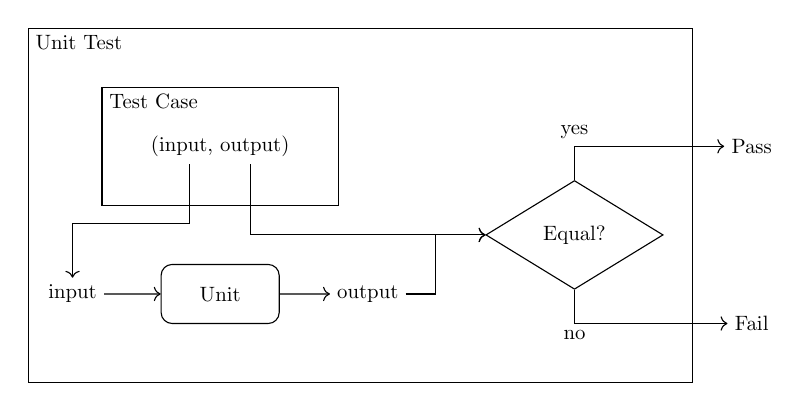
\begin{tikzpicture}[scale=.75,transform shape]

\tikzstyle{decision} = [diamond, minimum width=3cm, minimum height=1cm, text centered, draw=black]

\node[below right] (testcase) at (-1.25,6) {Unit Test};
\draw (-1.25,6) rectangle (10, 0);

\node[below right] (testcase) at (0,5) {Test Case};
\draw (0,5) rectangle (4, 3);
\node (tcInput) at (2,4) {(input, output)};

\node[draw,rounded corners,minimum width=2cm, minimum height=1cm] (unit) at (2, 1.5) {Unit};
\node[left of=unit,xshift=-1.5cm] (input) {input};
\node[right of=unit,xshift=1.5cm] (output) {output};

\node[decision] (equal) at (8, 2.5) {Equal?};

\node[] (pass) at (11, 4) {Pass};
\node[] (fail) at (11, 1) {Fail};

\draw[->] (input) -- (unit);
\draw[->] (unit) -- (output);


\draw[->] (tcInput.210) |- ++(0,-1) -| (input.north);
\draw[->] (tcInput.330) |-  (equal.west);
\draw[->] (output.east) -| ++(.5,0) |-  (equal.west);

\draw[->] (equal.north) |- node[pos=.5,above] {yes} (pass.west);
\draw[->] (equal.south) |- node[pos=.5,below] {no} (fail.west);

\end{tikzpicture}
\end{center}


\end{frame}

\begin{frame}
    \frametitle{Importance of Testing}
    \framesubtitle{}

\begin{itemize}[<+->]
  \item Testing provides some \emph{assurance of quality}
  \item Provide a reasonably high confidence that our software is \emph{correct}
  \item Correct: it conforms to our specifications or expectations
  \item Never a guarantee: testing only gives assurances for 
    what we test, not for what we do not (or cannot) test 
  \item Still possible to have false positives and false 
    negatives if our tests are wrong
  \item Prevents/reduces costly bugs that manifest themselves ``in production''
  \item Informs good design
\end{itemize}

\end{frame}

\begin{frame}
    \frametitle{Goals of Testing}
    \framesubtitle{}

\begin{itemize}[<+->]
  \item Should strive for good or high \emph{code coverage}
  \item Test as many types of input(s) as we can
  \item Edge cases: testing ``extreme'' inputs or input 
    values at the edge of extreme
  \item Corner cases: outside normal operating procedures 
    %(does our error checking work?)
  \item Try to break our code; be \emph{adversarial}
  %\item Fuzzing: providing invalid or random data to test recovery/error handling
  \item Don't just test what you expect should work
\end{itemize}

\end{frame}

\begin{frame}
    \frametitle{Costs of Testing}
    \framesubtitle{}

\begin{itemize}[<+->]  
  \item Testing code is often larger than the code it tests
  \item May require just as much or more time and effort as the code itself
  \item Example: SQLite is small (128.9 kLOC) but has 91,772 kLOC of testing code and scripts (711 times larger)
  %https://www.sqlite.org/testing.html
  \item Example: International Space Station has 1.8 mLOC vs 3.3 + 11 mLOC for simulation and testing
  \item Worth it: reduces \emph{technical debt}
  \item Testing is an \emph{investment}
  %\item Continuous Integration (CI)
  %\item Test Driven Development (TDD)
\end{itemize}  

\end{frame}

\begin{frame}
    \frametitle{Demonstration}
    \framesubtitle{}

%  HW1 updates need to be done: dev is on CSE:/CS1/KaprekarProject
%  Video: CSE:/CS1/cmockaDev (distance examples)

\begin{itemize}
  \item Ad-hoc Testing %testing via command line, as you develop
  \item Designing a suite of automated tests
  \item Unit testing with a formal testing framework: cmocka
\end{itemize}

\end{frame}



\end{document} 
